\section{Introduction}

\subsection{Cross-DC Erasure Coding: Why Now?}

As the entire IT industry is rapidly moving to the cloud, more and more data centers are being built all over the globe. The event that one of the data centers will fail catastrophically gradually becomes inevitable. In other words, this is no longer a matter of ``if'', but rather ''when''. {\em Designing for disasters}~\cite{bib:disasters} becomes essential and data stored in the cloud have to be protected against catastrophic failure.

There have been a long line of prior work~\ref{bib:BlahBlah} arguing for storing data objects in erasure coded form, as opposed to replication, across geo-graphically distributed data centers. Similar to geo-replication, cross-DC erasure coding can ensure durability even in the event of catastrophic data center failure. A main motivation for cross-DC erasure coding is to significantly reduce storage cost compared to geo-replication. The same economic force that has driven cloud providers to erasure code data within individual data centers naturally extends to the cross-DC scenario.

Nevertheless, none of the cloud providers today offer options to erasure code customer data across data centers. This is largely due to the prohibitive cost of WAN bandwidth. The reduction in storage cost of cross-DC erasure coding comes at the additional cost of inflated WAN traffic, for both read/write during normal operation and access/rebuild in the event of data center failure, as illustrated in detail in section~\ref{sec:motivation}.
Since the total cost of cloud storage includes both the storage cost in individual data centers and the WAN traffic cost across the data centers, cross-DC erasure coding has not become an economic solution yet.

Fortunately, the technology advancement in wide area networking has progressed to a point where new innovations have greatly reduced WAN bandwidth cost. There are two key driving forces: 1) The erbium-doped fiber amplifiers~\cite{mears1986low} make it practical to amplify a huge spectrum of optical signal directly, without the need to first convert it to an electrical signal. 2) Dense Wave Division Multiplexing (DWDM) is therefore enabled by the fiber amplifiers and can send 10+ terabits per single fiber~\cite{zhu2011112}.

Most recently, Facebook and Microsoft have teamed up to build $MAREA$, a new fiber optic cable under the Atlantic Ocean that uses eight pairs of fiber optic strands and will come online in 2017 with 160 Tbps capacity~\cite{bib:MAREA1, bib:MAREA2}. Compared to MAREA, another transatlantic cable, FLAG Atlantic 1~\cite{bib:FA-1}, had a mere capacity of 10 Gbps when coming online in 2001. The over 10,000x bandwidth increase in less than two decades is summarized in Table~\ref{tab:mears}. While the cost of MAREA remains undisclosed, it suffices to show that the cost of WAN bandwidth has reduced by several orders of magnitude. Indeed, the significant cost reduction in WAN bandwidth now makes cross-DC erasure coding economically attractive. And Project Giza addresses technical challenges so as to make such economical solution a reality.

\begin{table}[thp]
\centering
\begin{tabular}{|l|c|c|}
\hline
TransAtlantic Cable             & FLAG Atlantic 1~\cite{bib:FA-1}   & MAREA~\cite{bib:MAREA1, bib:MAREA2}
\\ \hline \hline
Ready For Service               & 2001                              & 2017
\\ \hline
Cost (Billion)                  & 1.1                               & undisclosed
\\ \hline
Capacity                        & 10 Gbps                           & 160 Tbps
\\ \hline \hline
\end{tabular}
\caption{Cost of WAN bandwidth reduced by orders of magnitude.}
\label{tab:mears}
\end{table}

\comment{bib:MAREA1, http://www.wsj.com/articles/facebook-and-microsoft-to-build-fiber-optic-cable-across-atlantic-1464298853}
\comment{bib:MAREA2, http://www.usatoday.com/story/experience/2016/05/26/microsoft-facebook-undersea-cable-google-marea-amazon/84984882/}
\comment{bib:FA-1, https://en.wikipedia.org/wiki/Fiber-Optic_Link_Around_the_Globe}

\subsection{Giza Overview}

Giza provides an externally consistent (linearizable~\cite{herlihy1990linearizability}) versioned cloud storage service, which erasure codes data objects and stores them across globally distributed data centers.

Customers access Giza service by creating Giza storage accounts. Per storage account, Giza allows the customers to specify the set of data centers where their data are striped across. In addition, the customers have the flexibility to choose erasure coding scheme. Giza employs classic $n = k + r$ Reed-Solomon coding, which generates $r$ parity fragments from $k$ data fragments. All $n$ fragments are stored in different data centers, where 1) failures of up to $r$ arbitrary data centers are tolerated; and 2) data can be reconstructed from any $k$ out of the $n$ data centers. By allowing the customers to specify the set of data centers and choose the erasure coding scheme, Giza gives the customers complete control of durability and storage overhead.

The customers access Giza with straightforward {\em put}/{\em get}/{\em delete} interface. In addition, Giza provides optional support of versioning, where new {\em put} does not overwrite existing data, but rather creates a new version of the same data. The old version remains available until it is explicitly expired or deleted.

Giza operates on the top of existing cloud storage system and leverages public APIs. It uses blob storage to store customer data and NoSQL table storage to store metadata.

\begin{figure}[tp]
\centering
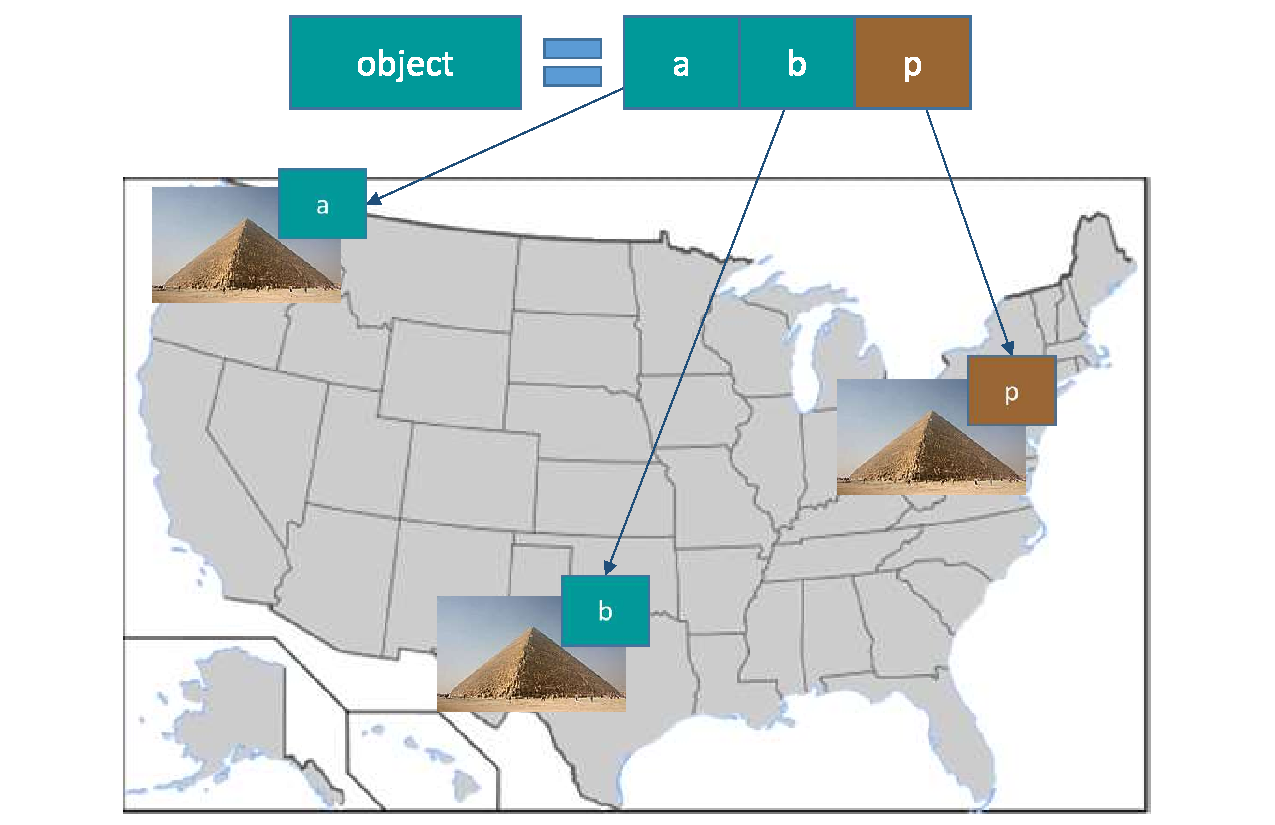
\includegraphics[width=0.5\textwidth]{images/giza_example_crop_fit}
\caption{Store Object in Giza}
\end{figure}

Figure~\ref{fig:giza_example} illustrates the flow of storing a customer data object. Giza operates a number of {\em stateless} Giza nodes in every data center. Say a customer uses a Giza client (command line, library, or REST interface) to store a 4MB data object. The Giza client routes the {\em put} request to one of the Giza nodes in the data center closest to the customer. The Giza node divides the data object into $2$ data fragments ($a$ and $b$) of 2MB each. It then invokes erasure coding and generates a parity fragment $p$ of size 2MB. The Giza node stores all the $3$ fragments (2 data and 1 parity) in the blob storage in 3 data centers (1 local and 2 remote). It also stores the metadata, consisting of the pointers to the blob storage, as well as versioning information, in the NoSQL table storage in the 3 data centers.

\subsection{Challenges and Contributions}

The target workloads for Giza are large data objects in cloud drives, such as Dropbox, Microsoft OneDrive, Google Drive, etc. The common properties of such workloads include: 1) large storage space consumption, 2) relatively cold data, where a small percentage of data is occasionally accessed across large volumes, 3) objects may be updated over time, but concurrent updates of the same object is very rare (but possible).

Given the target workloads, Giza optimizes for the common case, where there is single writer (and multiple readers). Giza strives to {\em make the common case fast}. In fact, the most optimized version of Giza achieves optimal write latency, which is single WAN RTT for {\em put}.

On the other hand, Giza does handle concurrency properly, which could arise in various situations. For instance, Giza tolerates data center failure. In the event of one or multiple data centers become temporarily unavailable (or simply slow), the customer are able to continue to read and write data objects without much impact. The unavailable (or slow) data centers may miss updates, which could potentially lead to conflict when receiving new updates again. Also, retry of {\em put} operation could be routed to a different DC and therefore conflict with the previously unfinished {\em put}. Therefore, even though concurrency is rare, it is crucial for Giza to {\em guarantee the rare case correct}. Indeed, Giza provides external consistency (linearizability).

Giza operates on the top of existing cloud storage system. It stores data in blob storage and metadata in NoSQL table storage across multiple data centers. The blob storage and NoSQL table storage within individual data centers operate independently. Hence, while strongly consistent individually, the collection of blob and table storage across DCs do not readily offer the desired linearizability. The key technical challenge Giza addresses is how to achieve optimal {\em put} latency with single writer, while at the same time provide linearizability under concurrency, over the collection of individual blob and table storage across multiple DCs.

Towards this end, the paper makes the following contributions:
\begin{itemize}
    \item We have designed and implemented Giza, which provides a versioned object store that erasure codes data objects and stores them across globally distributed data centers.
    \item Giza is fast in the common case: when there is no concurrency, Giza completes within single WAN RTT, which is optimal given the requirement to tolerate data center failure.
    \item Giza is correct when accessed concurrently: even with data center failure, Giza achieves external consistency.
    \item Giza employs well-known distributed algorithms, such as Paxos and Fast Paxos, in a novel way so that it operates on the top of existing public cloud storage systems.
    \item Giza is deployed in xxx data centers. Trace-driven experiments demonstrate that Giza achieve all our design goals. In particular, it is worth pointing out that Giza achieves much lower latency than naively adopting a globally consistent storage system, like CockroachDB (open source implementation of Google's spanner).
\end{itemize}
